\section{Issues with unidirectionality of AR models in STR}

As discussed in the main text, the unidirectionality of AR models could result in spurious addition of suffixes and direction-dependent decoding. Shown in \Cref{tab:spurious-suffixes} is a sample output of a \textit{left-to-right} (LTR) AR model trained on a 36-character lowercase charset. Since the input is fairly clear and horizontal, the model was very confident in the predictions for the first 10 characters. However, since it was trained on alphanumeric characters only, it did not know how to recognize the exclamation mark. The language context \textit{swayed} the output of the model to add the \textit{-ly} suffix in order to make sense of the unrecognized character. A \textit{right-to-left} (RTL) AR model would not add the suffix due to the lack of context (since the right-most characters would have to be predicted first). This direction-dependent decoding is further illustrated in \Cref{tab:direction-dependent} where two AR models trained on opposing directions produce different outputs. In this case, the input contains ambiguity on the uppercase \textit{N} character. If read from left to right, the context of the earlier characters can be used to infer that the ambiguous character is \textit{N}. However, when read in the opposite direction, the context of \textit{OPE} is not yet available, prompting the RTL model to recognize two \textit{l}'s in place of a single \textit{N} character.

\begin{table}[htbp]
    \centering
    \setlength{\tabcolsep}{5pt}
    \caption{Example of a spurious suffix from a left-to-right AR model. \textit{GT} refers to the ground truth label, while \textit{Confidence} pertains to per-character prediction confidence}
    \label{tab:spurious-suffixes}
    \begin{tabular}{c c | c c}
        \toprule
         Input & GT & Prediction & Confidence  \\
        \midrule
         \includegraphics[width=1in]{TERRIFYING.png} & terrifying & terrifying\textcolor{red}{ly} & [1.00, \dots, 1.00, 0.97, 0.72] \\
        \bottomrule
    \end{tabular}
\end{table}

\begin{table}[htbp]
    \centering
    \setlength{\tabcolsep}{5pt}
    \caption{Example of direction-dependent decoding with two AR models}
    \label{tab:direction-dependent}
    \begin{tabular}{c c | c c c}
        \toprule
        Input & GT & Direction & Prediction & Confidence \\
        \midrule
        \multirow{2}{*}{\includegraphics[width=0.8in]{open.png}} & \multirow{2}{*}{open} & LTR & open & [1.00, 1.00, 1.00, 0.66] \\
        & & RTL & ope\textcolor{red}{ll} & [1.00, 1.00, 0.52, 0.57, 0.94] \\
        \bottomrule
    \end{tabular}
\end{table}


\section{Inefficiency of External Language Models in STR}

As mentioned in the main text, ensemble methods such as ABINet \cite{Fang_2021_CVPR} and SRN \cite{yu2020towards} utilize a standalone or external Language Model (LM). In \Cref{tab:external-lm}, we show the cost measurements of \texttt{fvcore} on the full ABINet model for a single input, as well as the measurement breakdown for its component models. We can see that while the LM accounts for around 34.48\% of the parameter count, it only uses 13.65\% of the overall FLOPS and 15.78\% of the overall activations (a measure shown to be correlated with model runtime \cite{dollar2021fast,xiao2021early}). When evaluated in spelling correction on the 36-character set, the LM achieves a top-5 word accuracy of only 41.9\% \cite{Fang_2021_CVPR}. With the ground truth label itself as input (\Cref{tab:abinet-lm-acc}), the same model gets a top-1 word accuracy of only 50.44\% (36-char). This means that even if the Vision Model (VM) is perfect (always predicting the correct label), the LM will produce a wrong output 50\% of the time. In summary, the external LM's dedicated compute cost, underutilization relative to its parameter and memory requirements, and dismal word accuracy show the inefficiency of this approach. For STR, an internal LM might be more appropriate since the primary input signal is the image, not the language context.

\begin{table}[htbp]
    \setlength{\tabcolsep}{6pt}
    \centering
    \fontsize{8}{9.6}\selectfont
    \caption{Commonly used cost indicators as measured by \texttt{fvcore} for ABINet. \textit{Full Model} pertains to the overall measurements}
    \label{tab:external-lm}
    \begin{tabular}{l|r r r}
        \toprule
        \textbf{Module} & \# of Parameters (M) & FLOPS (G) & \# of Activations (M) \\
        \midrule
        Full Model & 36.858 \textit{(100.00\%)} & 7.289 \textit{(100.00\%)} & 10.785 \textit{(100.00\%)} \\
        \midrule
        - Vision & 23.577 \textit{(63.97\%)} & 6.249 \textit{(85.73\%)} & 9.036 \textit{(83.78\%)} \\
        - Language & 12.707 \textit{(34.48\%)} & 0.995 \textit{(13.65\%)} & 1.702 \textit{(15.78\%)} \\
        - Alignment & 0.574 \textit{(1.55\%)} & 0.045 \textit{(0.62\%)} & 0.047 \textit{(0.44\%)} \\
        \bottomrule
    \end{tabular}
\end{table}

\begin{table}[htbp]
    \centering
    \fontsize{8}{9.6}\selectfont
    \caption{Performance of ABINet's LM when the ground truth label itself is used as the input}
    \begin{tabular}{c|r|r|r}
        \toprule
        Dataset & \# of samples & Word acc. (\%) & 1 - NED \\
        \midrule
        IIIT5k & 3,000 & 47.33 & 69.50 \\
        SVT & 647 & 65.38 & 83.48 \\
        IC13 & 1,015 & 62.07 & 78.77 \\
        IC15 & 2,077 & 40.49 & 67.72 \\
        SVTP & 645 & 65.27 & 83.08 \\
        CUTE80 & 288 & 46.88 & 68.65 \\
        \midrule
        \textbf{Combined} & \textbf{7,672} & \textbf{50.44} & \textbf{72.54} \\
        \bottomrule
    \end{tabular}
    \label{tab:abinet-lm-acc}
\end{table}


\section{Multi-head Attention}

The attention mechanism is central to the operation of Transformers \cite{vaswani2017attention}. In scaled dot-product attention, the similarity scores between two $d_k$-dimensional vectors $\mathbf{q}$ (query) and $\mathbf{k}$ (key), computed using their dot-product, are used to transform a $d_v$-dimensional vector $\mathbf{v}$ (value). Formally, scaled dot-product attention is defined as:

\begin{equation}
  Attn(\mathbf{q}, \mathbf{k}, \mathbf{v}) = softmax \left( \frac{\mathbf{q}\mathbf{k}^T}{\sqrt{d_k}} \right) \mathbf{v}
  \label{eq:sdpattn}
\end{equation}It accepts an optional \textit{attention mask} that limits which \textit{keys} the \textit{queries} could attend to. In a Transformer with token dimensionality of $d_{model}$, $d_k = d_v = d_{model}$.

Multi-head Attention (MHA) is the extension of scaled dot-product attention to multiple representation subspaces or \textit{heads}. To keep the computational cost of MHA practically constant regardless of the number of heads, the dimensionality of the vectors are reduced to $d_{head} = d_{model} / h$, where $h$ is the number of heads. A \textit{head} corresponds to an invocation of \Cref{eq:sdpattn} on projected versions of $\mathbf{q}$, $\mathbf{k}$, and $\mathbf{v}$ using parameter matrices $\mathbf{W}^q \in \mathbb{R}^{d_{model}\times{d_{head}}}$, $\mathbf{W}^k \in \mathbb{R}^{d_{model}\times{d_{head}}}$, and $\mathbf{W}^v \in \mathbb{R}^{d_{model}\times{d_{head}}}$, respectively, as shown in \Cref{eq:attn_head}. The final output is obtained in \Cref{eq:mha} by concatenating the heads and multiplying by the output projection matrix $\mathbf{W}^o \in \mathbb{R}^{{d_{model}}\times{d_{model}}}$.

\begin{equation}
    head_i = Attn(\mathbf{q}\mathbf{W}^q_i, \mathbf{k}\mathbf{W}^k_i, \mathbf{v}\mathbf{W}^v_i)
    \label{eq:attn_head}
\end{equation}

\begin{equation}
    MHA(\mathbf{q}, \mathbf{k}, \mathbf{v}) = Concat(head_1, ..., head_h)\mathbf{W}^o
  \label{eq:mha}
\end{equation}


\section{Model Architecture}
\label{ch:arch-appendix}

PARSeq uses an encoder which largely follows the original ViT \cite{dosovitskiy2020image}, and a pre-$LayerNorm$ \cite{baevski2018adaptive,wang2019learning} decoder with more heads. The architectures are practically unchanged but are reproduced here for the convenience of the reader.

\subsection{ViT Encoder}

The encoder is composed of 12 layers. All layers share the same architecture shown in \Cref{fig:vit-arch}. The output of the last encoder layer goes through a final $LayerNorm$.

\begin{figure}[ht]
  \centering
  \includegraphics[height=0.58\linewidth]{vit-layer.png}
   \caption[Illustration of a ViT layer.]{Illustration of a ViT layer from Dosovitskiy \etal \cite{dosovitskiy2020image}. \textit{Norm} pertains to $LayerNorm$.}
   \label{fig:vit-arch}
\end{figure}

\subsection{Visio-lingual Decoder}

The decoder (\Cref{fig:decoder-arch-detailed}) consists of only a single layer. The immediate outputs of all $MHA$ and $MLP$ layers go through $Dropout$ ($p = 0.1$, not shown). \textit{Image Features} are already $LayerNorm$'d by the encoder (hence no $LayerNorm$ prior to input).

\begin{figure}[ht]
  \centering  \includegraphics[width=0.98\linewidth]{decoder-arch-detailed.png}
   \caption{Visio-lingual decoder architecture with $LayerNorm$ layers shown.}
   \label{fig:decoder-arch-detailed}
\end{figure}

\subsection{Architecture Configuration}
\label{sec:arch-config}

The main results are obtained from the base model, PARSeq-S, which has a similar configuration to DeiT-S \cite{touvron2021training} but uses an image size of 128$\times$32 and a patch size of 8$\times$4 (a change also adapted in our reproduction of ViTSTR-S). Based on our experiments, scaling up the model only marginally improves word accuracy on the benchmark. We instead explore scaling down the model to make it more suitable for edge devices. PARSeq-Ti, which uses a configuration similar to DeiT-Ti \cite{touvron2021training}, is more similar to CRNN \cite{shi2016end} in terms of parameter count and FLOPS. The detailed configuration parameters are shown in \Cref{tab:arch-config}.

\begin{table}[ht]
  \centering
  \setlength{\tabcolsep}{8pt}
  \caption[Configurations for PARSeq-S and PARSeq-Ti model variants.]{Configurations for the base (PARSeq-S) and smaller (PARSeq-Ti) model variants. $d_{model}$ refers to the \textit{dimensionality} of the model which dictates the dimensions of the vectors and feature maps. $h$ refers to the number of \textit{attention heads} used in MHA layers. $d_{MLP}$ refers to the dimension of the intermediate features within the MLP layer. \textit{depth} refers to the number of encoder or decoder layers used}
  \begin{tabular}{c|c|c c c|c c c}
    \toprule
    & & \multicolumn{3}{c}{\textit{encoder}} & \multicolumn{3}{c}{\textit{decoder}} \\
    \textbf{Variants} & $d_{model}$ & $h$ & $d_{MLP}$ &
      depth & $h$ & $d_{MLP}$ & depth \\
    \midrule
      PARSeq-Ti & 192 & 3 & 768 & 12 & 6 & 768 & 1 \\
      PARSeq-S & 384 & 6 & 1536 & 12 & 12 & 1536 & 1 \\
    \bottomrule
  \end{tabular}
  \label{tab:arch-config}
\end{table}


\section{Permutation Language Modeling}
\label{sec:plm-appendix}

In this section, we provide additional details about the adaptation of PLM for use in PARSeq. We give a concrete illustration of masked multi-head attention first. Next, the intuition behind the usage of permutation pairs is discussed. Lastly, implementation details and considerations about the training procedure are discussed.

\subsection{Illustration of attention masking}

As discussed in the main text, Transformers process all tokens in parallel. In order to enforce the \textit{AR} constraint which limits the conditional dependencies for each token, attention masking is used. \Cref{fig:attn-connectivity} shows a concrete example of masked multi-head attention for a sequence $\mathbf{y}$. The \textit{position} tokens always serve as the \textit{query} vectors, while the \textit{context} tokens (context \textit{embeddings} with position information) serve as the \textit{key} and \textit{value} vectors. Note that the sequence order is \textit{fixed}, and that only the AR factorization order (specified by the attention mask) is permuted.

\begin{figure}[htbp]
  \centering
    \subfloat[MHA for output token $y_1$]{\centering
         \includegraphics[width=0.45\textwidth]{attention-connectivity-y1.png}
         \label{fig:attn-connectivity:y1}
    }
    \hfill
    \subfloat[MHA for output token $y_2$]{\centering
         \includegraphics[width=0.45\textwidth]{attention-connectivity-y2.png}
         \label{fig:attn-connectivity:y2}
     }
     \hfill
     \subfloat[MHA for output token $y_3$]{\centering
         \includegraphics[width=0.45\textwidth]{attention-connectivity-y3.png}
         \label{fig:attn-connectivity:y3}
     }
    \hfill
    \subfloat[MHA for output token \texttt{[E]}]{\centering
         \includegraphics[width=0.45\textwidth]{attention-connectivity-eos.png}
         \label{fig:attn-connectivity:eos}
     }
     
     \caption{Masked MHA for a three-element sequence $\mathbf{y} = [y_1, y_2, y_3]$ given the factorization order $[1, 3, 2]$. $\mathbf{c}$ are context embeddings with position information}
    \label{fig:attn-connectivity}
\end{figure}

\subsection{Permutation Sampling}
\label{sec:perm-sampling}

As discussed in the main text, we sample permutations in a specific way. We use pairs of permutations, and the \textit{left-to-right} permutation is always used. Thus, we only sample $K / 2 - 1$ permutations every training step. To illustrate the intuition behind the usage of \textit{flipped} permutation pairs, we give the following example. Given a three-element text label $\mathbf{y} = [y_1, y_2, y_3]$ and $K = 4$ permutations: $[1, 2, 3]$, $[3, 2, 1]$, $[1, 3, 2]$, and $[2, 3, 1]$. The first two permutations are the \textit{left-to-right} and \textit{right-to-left} orderings, respectively. Both are always used as long as $K > 1$. The corresponding factorizations of the joint probability per pair are as follows:

\begin{align*}
    p(\mathbf{y})_{[1, 2, 3]} &= p(y_1) p(y_2 | y_1) p(y_3 | y_1, y_2) \\
    p(\mathbf{y})_{[3, 2, 1]} &= p(y_3) p(y_2 | y_3) p(y_1 | y_2, y_3)
\end{align*}
    
\begin{align*}
    p(\mathbf{y})_{[1, 3, 2]} &= p(y_1) p(y_3 | y_1) p(y_2 | y_1, y_3) \\
    p(\mathbf{y})_{[2, 3, 1]} &= p(y_2) p(y_3 | y_2) p(y_1 | y_2, y_3)
\end{align*}

For each permutation pair, if we group the probabilities per element, we get \Cref{tab:grouped-probs}. Notice that the probabilities of each element for every permutation pair consists of disjoint sets of conditioning variables. For example, the probabilities of element $y_1$ for $[1,2,3]$  (\textit{left-to-right} permutation) and $[3,2,1]$ (\textit{right-to-left} permutation) are $p(y_1)$ and $p(y_1 | y_2, y_3)$, respectively. The first term is the prior probability of $y_1$. It is not conditioned on any other element of the text label, unlike the second term which is conditioned on all other elements, $y_2$ and $y_3$. Similarly for $y_2$, the first term is conditioned only on $y_1$ while the second term is conditioned only on $y_3$. In our experiments, we find that using flipped permutation pairs results in more stable training dynamics where the loss is smoother and less erratic.

\begin{table}[ht]
  \centering
  \setlength{\tabcolsep}{6pt}
  \caption{Probability terms grouped by permutation pairs.}
  \begin{tabular}{ c | l l l }
    \toprule
    Perm. & $y_1$ & $y_2$ & $y_3$ \\
    \midrule
    $[1,2,3]$ & $p(y_1)$ & $p(y_2 | y_1)$ & $p(y_3 | y_1, y_2)$ \\
    $[3,2,1]$ & $p(y_1 | y_2, y_3)$ & $p(y_2 | y_3)$ & $p(y_3)$ \\
    \midrule
    $[1,3,2]$ & $p(y_1)$ & $p(y_2 | y_1, y_3)$ & $p(y_3 | y_1)$ \\
    $[2,3,1]$ & $p(y_1 | y_2, y_3)$ & $p(y_2)$ & $p(y_3 | y_2)$ \\
    \bottomrule
  \end{tabular}
  \label{tab:grouped-probs}
\end{table}






\subsection{Special handling of end-of-sequence \texttt{[E]} token}

Although the \texttt{[E]} token is part of the sequence, it is handled in a specific way in order to make training simpler. First, no character $c \in C$, where $C$ is the training charset, is conditioned on \texttt{[E]}. Intuitively, it means that \texttt{[E]} marks the end of the sequence (hence its name) since no more characters are expected after it is produced by the model. More formally, it means that $p(c | \texttt{[E]}) = 0$. This is achieved by masking the positions of \texttt{[E]} in the input context. Second, we train \texttt{[E]} on only two permutations, \textit{left-to-right} and \textit{right-to-left}. The \textit{left-to-right} lookahead mask provides the longest context to \texttt{[E]} (conditioned on all other characters in the sequence), while the \textit{right-to-left} mask provides no context, which is necessary for NAR decoding. We could also train \texttt{[E]} on different subsets of the input context, but doing so needlessly complicates the training procedure without offering any advantages.

\subsection{Considerations for batched training}

Text labels of varying lengths can be included in a mini-batch. However, the sampled permutations for the mini-batch are always based on the longest sequence. Hence, it is possible that after accounting for padding, multiple permutations would become equivalent. To see why this is the case, consider a mini-batch containing two samples: the first label has a single character, while the second label has four characters. The first label has a sequence length of one and total number of permutations also equal to one. On the other hand, the second label has a sequence length of four which corresponds to 24 total permutations. If we use $K = 6$ permutations, then it means that the permutations for the first label would be oversampled since there is only one valid permutation for $T = 1$. We find that this oversampling actually helps training. We experimented with a modified training procedure wherein sequences with $T < 4$ are grouped together (\ie 1-, 2-, and 3-character sequences are grouped separately). This training procedure results in increased training time due to the mini-batch being split further into smaller batches, but it does not improve accuracy nor hasten convergence. Thus, we stick with the simpler batched training procedure.

\section{Dataset Matters}

\subsection{Open Images Datasets}
\label{ch:open-images}

TextOCR and OpenVINO are datasets both derived from Open Images---a large dataset with very diverse images often containing complex scenes with several objects (8.4 per image on average). Open Images is not specifically collected for STR. Thus, it contains text of varying resolutions, orientations, and quality, as shown in cropped word boxes in \Cref{fig:open-images-cropped-words}. TextOCR and OpenVINO significantly overlap in terms of source scene images, as shown in \Cref{tab:textocr-openvino-overlap}. Samples of source scene images common to both are shown in \Cref{fig:textocr-openvino-overlap}. Only the 
\textit{validation} set of OpenVINO and the \textit{test} set of TextOCR do not overlap any other image set. The labels of TextOCR's \textit{test} set are kept private.

\begin{figure}[htbp]
  \centering
  \includegraphics[width=0.9\linewidth]{textocr-samples.png}
   \caption{Cropped word boxes from Open Images.}
   \label{fig:open-images-cropped-words}
\end{figure}

\begin{table}[htbp]
  \centering
  \setlength{\tabcolsep}{10pt}
  \caption{Overlap between TextOCR and OpenVINO in terms of the number of common source scene images.}
  \begin{tabular}{ c c | r r r }
    \toprule
    & & \multicolumn{3}{c}{\textbf{TextOCR}} \\
    & & train & val & test \\
    \midrule
    \multirow{5}{*}{\rotatebox[origin=c]{90}{\textbf{OpenVINO}}} & train\_1 & 1,612 & 225 & 0 \\
    & train\_2 & 1,444 & 230 & 0 \\
    & train\_5 & 1,302 & 184 & 0 \\
    & train\_f & 1,068 & 157 & 0 \\
    & validation & 0 & 0 & 0 \\
    \bottomrule
  \end{tabular}
  \label{tab:textocr-openvino-overlap}
\end{table}

\begin{figure*}[htbp]
  \centering
  \includegraphics[width=\linewidth]{textocr-openvino-common.png}
   \caption{Examples of source scene images common to TextOCR and OpenVINO.}
   \label{fig:textocr-openvino-overlap}
\end{figure*}

\subsection{Data preparation for LMDB storage}

We use the archives released by Baek \etal \cite{Baek_2021_CVPR} for RCTW17, Uber-Text, ArT, LSVT, MLT19, and ReCTS. Thus, we only preprocess data for the remaining datasets.

For COCO-Text, we use the v1.4 \textit{test} annotations released as part of the ICDAR 2017 challenge. For \textit{train} and \textit{val}, we use the latest (v2.0) annotations. We preprocess TextOCR, OpenVINO, and COCO-Text with minimal filtering and modifications, in contrast to the usual practice of removing non-horizontal text and special characters. We only filter illegible and non-machine printed text. The only modification we perform is the removal of whitespace on either side of the label, or duplicate whitespace between non-whitespace characters.

For IC13 and IC15, we use the original data from the ICDAR competition website and perform no modifications to the data. We emulate the previous filtering methods \cite{wang2011end,cheng2017focusing} to create the subsets used for evaluation.

Long and Yao \cite{long2020unreal} have reannotated IIIT5k, CUTE, SVT, and SVTP because the original annotations are case-insensitive and lack punctuation marks. However, both the reannotations and the originals contain some errors. Hence, we review inconsistencies between the two versions and manually reconcile them to correct the errors.

\Cref{tab:dataset} provides a detailed summary of how each dataset was used.

\begin{table}[htbp]
  \centering
  \fontsize{6.5}{7.8}\selectfont
  \caption{Summary of dataset usage after on-the-fly filtering for the 94-character set. Numbers indicate how many samples were used from each dataset. \textsuperscript{t} and \textsuperscript{v} refer to splits that were repurposed as training and validation data, respectively. \textsuperscript{*} indicates private ground truth labels. -- indicates that the dataset does not have a particular split. IC13 and IC15 have two \textit{versions} of their respective \textit{test} splits commonly used in the literature.}
  \setlength{\tabcolsep}{10pt}
  \begin{tabular}{ c | r r r }
    \toprule
    Dataset & \textit{train} & \textit{val} & \textit{test} \\
    \midrule
    MJSynth & 7,224,586 & 802,731\textsuperscript{t} & 891,924\textsuperscript{t} \\
    SynthText & 6,975,301 & -- & -- \\
    \midrule
    LSVT & 41,439 & -- & -- \\
    MLT19 & 56,727 & -- & -- \\
    RCTW17 & 10,284 & -- & -- \\
    ReCTS & 21,589 & -- & 2,467\textsuperscript{t} \\
    TextOCR & 710,994 & 107,093\textsuperscript{t} & 0\textsuperscript{*} \\
    OpenVINO & 1,912,784 & 158,757\textsuperscript{t} & -- \\
    \midrule
    ArT & 32,028 & -- & 35,149 \\
    COCO & 59,733 & 13,394\textsuperscript{t} & 9,825 \\
    Uber & 91,732 & 36,188\textsuperscript{t} & 80,587 \\
    \midrule
    IIIT5k & 2,000\textsuperscript{v} & -- & 3,000 \\
    SVT & 257\textsuperscript{v} & -- & 647 \\
    IC13 & 848\textsuperscript{v} & -- & 857 / 1,015 \\
    IC15 & 4,468\textsuperscript{v} & -- & 1,811 / 2,077 \\
    SVTP & -- & -- & 645 \\
    CUTE & -- & -- & 288 \\
    \bottomrule
  \end{tabular}
  \label{tab:dataset}
\end{table}


\section{Training Details}

In the main text, the 169,680 training iterations (batch size of 384) is equivalent to 20 epochs on the combined real training dataset (3,257,585 samples). The same exact number of training iterations is used when training on synthetic data (MJ+ST, 15.89M samples), resulting in just over 4 epochs of training. As shown in \Cref{tab:training-sched}, this training schedule is more than twice as long as Baek \etal \cite{Baek_2021_CVPR} but is still much shorter than ABINet's original training schedule of 8 epochs VM pretraining on MJ+ST, 80 epochs LM pretraining on WikiText-103, and 10 epochs full model training on MJ+ST. This explains why our reproduction of CRNN and TRBA obtain higher accuracy than the originals, and why ABINet gets a slightly lower (1.4\%) accuracy compared to the original results.

\begin{table}[htbp]
    \centering
    \setlength{\tabcolsep}{5pt}
    \caption{Training schedule comparison vs reproduced methods. Sorted from shortest to longest schedule based on the \textit{sample count} (essentially \textit{batch size} $\times$ \textit{number of iterations})}
    \label{tab:training-sched}
    \begin{tabular}{c r r | r}
        \toprule
        \textbf{Method} & \textbf{Batch size} & \textbf{\# of iterations} & \textbf{Sample count} (M) \\
        \midrule
        CRNN and TRBA \cite{Baek_2021_CVPR} & 128 & 200,000 & 25.6 \\
        ViTSTR \cite{atienza2021vitstr} & 192 & 300,000 & 57.6 \\
        \textit{Ours} & 384 & 169,680 & 65.2 \\
        ABINet (VM + full) \cite{Fang_2021_CVPR} & 384 &  745,074 & 286.1 \\
        ABINet (LM) \cite{Fang_2021_CVPR} & 4,096 & 1,688,720 & 6,917.0 \\
        \bottomrule
    \end{tabular}
\end{table}

\subsection{Label preprocessing}
Preprocessing and filtering are done as follows. Whitespace characters are removed from the labels. Unicode characters are normalized using the NFKD normalization form and then converted to ASCII. Next, labels longer than $T$ characters are filtered. Case-sensitivity is inferred from the charset. If all letters in the charset are lowercase, the label is transformed to its lowercase version. If the charset consists of purely uppercase letters, the label is converted to its uppercase version. If the charset is mixed-case, no case conversion is done. Lastly, all characters not specified in the charset are removed from the labels.

\subsection{Learning Rate Optimization}
\label{ch:learning-rates}

\begin{table}[htbp]
  \centering
  \fontsize{7}{8.4}\selectfont
  \setlength{\tabcolsep}{5pt}
  \caption[Learning rates used for training.]{Learning rates used for training. The \textit{Base LR} is the raw value set in the configuration, while the \textit{Effective LR} is the actual value used for training. During pretraining, \textit{ABINet (LM)} is used for ABINet's language model}
  \begin{tabular}{ c | r r }
    \toprule
    Model & Base LR & Effective LR \\
    \midrule
    CRNN & $5.10\times10^{-4}$ & $1.08\times10^{-3}$ \\
    ViTSTR-S & $8.90\times10^{-4}$ & $1.89\times10^{-3}$ \\
    TRBC & $1.00\times10^{-4}$ & $2.12\times10^{-4}$ \\
    TRBA & $6.90\times10^{-4}$ & $1.46\times10^{-3}$ \\
    ABINet (LM) & $3.00\times10^{-4}$ & $6.36\times10^{-4}$ \\
    ABINet & $3.40\times10^{-4}$ & $7.21\times10^{-4}$ \\
    PARSeq & $7.00\times10^{-4}$ & $1.48\times10^{-3}$ \\
    \bottomrule
  \end{tabular}
  \label{tab:learning-rates}
\end{table}

For fair comparison during evaluation, all training hyperparameters---except the learning rate---are kept constant across models. The learning rate is varied because different architectures and model sizes train differently \cite{li2020train}. Ray Tune \cite{liaw2018tune} was used to automatically search for the optimum maximum learning rate given the fixed training schedule. Specifically, we used a combination of Median Stopping \cite{Vizier} and Bayesian Optimization \cite{balandat2020botorch} to efficiently narrow down the configuration space. Finally, a grid search over the narrowed down learning rate range was performed with models trained to completion. The final learning rates used for training are shown in \Cref{tab:learning-rates}. The base learning rates are scaled using two multipliers: the DDP factor ($\sqrt{nGPU}$) and the batch size linear scaling rule ($bsize / 256$) \cite{goyal2017accurate}, where $nGPU$ refers to the number of GPUs used (\ie $nGPU = 2$ for a dual-GPU setup) and $bsize$ refers to the batch size (\ie $bsize = 384$).

\section{Accuracy of decoding schemes vs latency}
\label{sec:acc-vs-latency}

\Cref{fig:ablation-decoding} shows how the word accuracy and latency evolve as functions of the number of refinement iterations. For AR decoding, refinement iterations after the first provide negligible increase in accuracy. For NAR decoding, the accuracy increase becomes insignificant after the second iteration. Hence, we use one and two refinement iterations for the AR and NAR decoding schemes, respectively.

\begin{figure}[htbp]
  \centering

    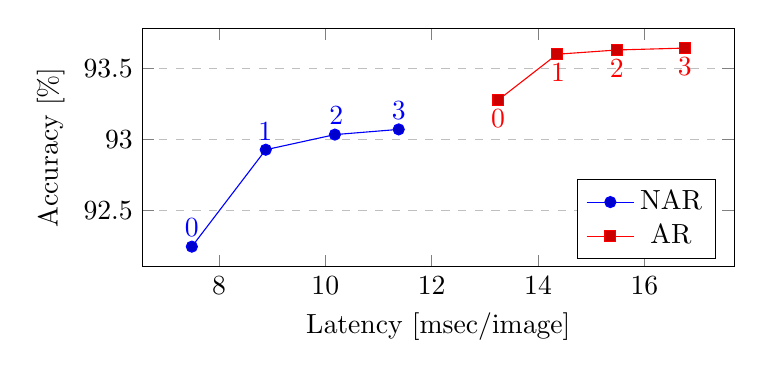
\begin{tikzpicture}
    \begin{axis}[
        ylabel={Accuracy [\%]},
        xlabel={Latency [msec/image]},
        legend pos=south east,
        ymajorgrids=true,
        grid style=dashed,
        cycle list name=color,
        width=0.75\linewidth,
        height=0.38\linewidth
    ]
    
    \addplot
        coordinates {
        (7.49,92.2433) (8.88,92.9267) (10.18,93.0333) (11.38,93.0700)
        } node[above, pos = 0] {0}
          node[above, pos = 0.38] {1}
          node[above, pos = 0.71] {2}
          node[above, pos = 1] {3}
          ;
        
    \addplot
        coordinates {
        (13.25,93.2767) (14.36,93.6000) (15.49,93.6300) (16.76,93.6433)
        } node[below, pos = 0] {0}
          node[below, pos = 0.33] {1}
          node[below, pos = 0.64] {2}
          node[below, pos = 1] {3}
          ;

    \legend{NAR,AR}

    \end{axis}
    \end{tikzpicture}

  \caption[PARSeq word accuracy and single-image latency for each decoding scheme.]{PARSeq word accuracy and single-image latency for each decoding scheme. The number of refinement iterations used is indicated for each point.}
  \label{fig:ablation-decoding}
\end{figure}

\section{Detailed Latency Measurements}
\label{ch:latency-measurements}

\begin{figure}[htbp]
  \centering

    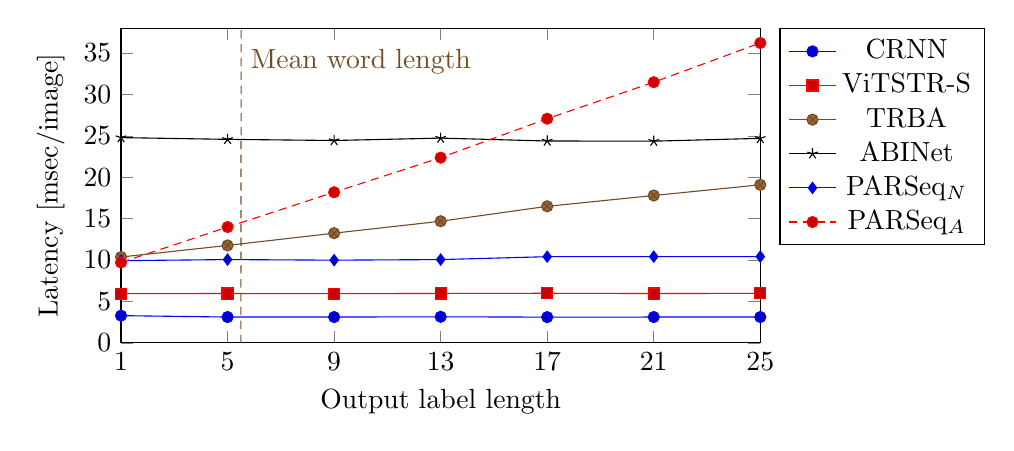
\begin{tikzpicture}
    \begin{axis}[
        xlabel={Output label length},
        ylabel={Latency [msec/image]},
        ymin=0, ymax=38,
        xmin=1, xmax=25,
        xtick={1, 5, 9, 13, 17, 21, 25},
        ytick={0, 5, 10, 15, 20, 25, 30, 35},
legend pos=outer north east,
grid style=dashed,
        cycle list name=color,
        width=0.8\linewidth,
        height=0.46\linewidth
    ]
    
    \addplot
        coordinates {
        (1,3.29) (5,3.12) (9,3.12) (13,3.15) (17,3.11) (21,3.12) (25,3.12)
        };
        
    \addplot
        coordinates {
        (1,5.95) (5,5.96) (9,5.94) (13,5.97) (17,5.99) (21,5.96) (25,5.98)
        };
    
    \addplot
        coordinates {
        (1,10.37) (5,11.77) (9,13.25) (13,14.69) (17,16.49) (21,17.80) (25,19.09)
        };
        
    \addplot
        coordinates {
        (1,24.79) (5,24.58) (9,24.44) (13,24.73) (17,24.38) (21,24.36) (25,24.70)
        };
        
    \addplot
        coordinates {
        (1,9.93) (5,10.06) (9,9.99) (13,10.06) (17,10.41) (21,10.41) (25,10.42)
        };
        
    \addplot
        coordinates {
        (1,9.71) (5,13.99) (9,18.19) (13,22.37) (17,27.07) (21,31.48) (25,36.22)
        };
        
    \addplot +[mark=none] coordinates {(5.5, 0) (5.51, 40)} node[right, pos = 0.85] {Mean word length};
    
    \legend{CRNN,ViTSTR-S,TRBA,ABINet,PARSeq$_{N}$,PARSeq$_{A}$}

    \end{axis}
    \end{tikzpicture}

  \caption[Model latency vs output label length.]{Model latency vs output label length as measured by PyTorch's benchmark timer on an NVIDIA Tesla A100 GPU. Each point corresponds to a mean of five runs of \texttt{Timer.blocked\_autorange()}. Lower is better. \textit{Mean word length} is the average length of the labels from all test datasets.}
  \label{fig:runtime}
\end{figure}

We measure model latency in an isolated manner. By doing so, we can reliably factor out the effects of data loading, storage, and CPU latency. We use the built-in benchmarking tool of PyTorch and measure latency for different label lengths, as shown in \Cref{fig:runtime}. As expected, NAR methods including PARSeq$_N$ exhibit near-constant latency regardless of output label length. Meanwhile, the latency of AR methods increases linearly as a function of the output label length. The latency increase of PARSeq$_A$ is steeper than TRBA. However, since the average length of words in the test datasets is quite short at 5.4, the actual difference in mean latency between TRBA and PARSeq$_A$ is only about 2.3 msec.

\section{Experiments on arbitrarily-oriented text}

In STR, the focus has mainly been on horizontal text, with a few explicitly tackling arbitrarily-oriented text \cite{phan2013recognizing,cheng2018aon,munjal2021stride,Yan_2021_CVPR,yan2021mean}. In our experiments, we observe that existing attention-based models are capable of recognizing text in arbitrary orientation, as shown in \Cref{tab:rotation-results}. Only CRNN, a CTC-based model, exhibits dismal orientation robustness. We conjecture that the direct correspondence of visual feature positions to textual feature positions in CTC-based models causes this poor performance. On the other hand, attention-based models compute feature similarity scores on-the-fly, resulting in a more dynamic alignment between visual and textual features.

\begin{table}[htbp]
  \centering
  \scriptsize
  \setlength{\tabcolsep}{5pt}
  \caption{Orientation robustness benchmark. Word accuracy (94-char) on rotated versions of the six benchmark datasets. \textit{\%dec} refers to the percentage decrease of the \textit{Mean} accuracy \wrt the 0\textdegree{} accuracy.}
  \begin{tabular}{ c | c | r r r | r r }
    \toprule
    Method & 0\textdegree$\uparrow$ & 90\textdegree$\uparrow$ & 180\textdegree$\uparrow$ & 270\textdegree$\uparrow$ & Mean$\uparrow$ & \%dec$\downarrow$ \\
    \midrule
    CRNN  & 85.8 & 11.8$\pm$0.1 & 6.4$\pm$0.5 & 10.7$\pm$0.2 & 9.6 & 88.8 \\
    ViTSTR-S & 91.8 & \textbf{87.9}$\pm$0.2 & 78.9$\pm$0.3 & 80.6$\pm$0.9 & 82.4 & 10.2 \\
    TRBA & 92.5 & 84.6$\pm$0.1 & 83.5$\pm$0.2 & 78.6$\pm$0.3 & 82.3 & 11.0 \\
    ABINet & 92.4 & 66.0$\pm$1.5 & 77.1$\pm$0.9 & 65.5$\pm$1.8 & 69.6 & 24.7 \\
    \midrule
    PARSeq$_{N}$ & 92.7 & 86.7$\pm$0.3 & 83.2$\pm$0.9 & 81.1$\pm$0.3 & 83.7 & 9.7 \\
    PARSeq$_{A}$ & \textbf{93.3} & \textbf{88.0}$\pm$0.1 & \textbf{86.6}$\pm$0.3 & \textbf{84.1}$\pm$0.1 & \textbf{86.2} & \textbf{7.6} \\
    \bottomrule
  \end{tabular}
  \label{tab:rotation-results}
\end{table}

We hypothesize that regardless of architecture and training procedure, the attention mechanism makes STR models generally robust against orientation variations. To test our hypothesis, we created a pose-corrected version of TextOCR which contains text in canonical orientation (practically horizontal), as opposed to the original version which contains text in arbitrary orientation. One possible contributor to the orientation robustness of TRBA is its image rectification module \cite{shi2016robust}. To test if this is the case, we also train TRBC, the CTC-based version of TRBA. We train all models on either TextOCR variants exclusively and show the results in \Cref{tab:horizontal-vs-arbitrary}.

\begin{table}[htbp]
  \centering
  \scriptsize
  \setlength{\tabcolsep}{10pt}
  \caption{Effect of training on horizontally-oriented (H) vs arbitrarily-oriented (A) variants of TextOCR. 0\textdegree{} pertains to model accuracy (94-char) on non-rotated benchmark datasets. \textit{Rotated} refers to the mean accuracy on 90\textdegree, 180\textdegree, and 270\textdegree{} rotations of the benchmark datasets. In H vs A per row, bold indicates significantly higher accuracy.}
  \begin{tabular}{ c | c c | c r }
    \toprule
    \multirow{2}{*}{Method} & \multicolumn{2}{c|}{0\textdegree{}} & \multicolumn{2}{c}{\textit{Rotated}} \\
    & H & A & H & A\hspace{14pt} \\
    \midrule
    CRNN & 84.7$\pm$0.4 & 84.0$\pm$0.4 & 0.8$\pm$0.0 & \textbf{8.7}$\pm$0.4 \\
    ViTSTR-S & 87.8$\pm$0.7 & 88.1$\pm$0.3 & 2.5$\pm$0.2 & \textbf{72.8}$\pm$1.3 \\
    TRBC & 87.0$\pm$0.2 & 87.3$\pm$0.2 & 1.3$\pm$0.1 & \textbf{17.3}$\pm$1.9 \\
    TRBA & 89.7$\pm$0.0 & \textbf{90.1}$\pm$0.2 & 2.7$\pm$0.1 & \textbf{76.3}$\pm$0.4 \\
    ABINet & 90.3$\pm$0.2 & 90.7$\pm$0.2 & 3.0$\pm$0.3 & \textbf{63.9}$\pm$1.5 \\
    \midrule
    PARSeq$_{N}$ & 89.8$\pm$0.3 & \textbf{90.4}$\pm$0.0 & 6.4$\pm$0.4 & \textbf{77.9}$\pm$0.6 \\
    PARSeq$_{A}$ & 90.6$\pm$0.0 & \textbf{91.3}$\pm$0.2 & 8.4$\pm$0.4 & \textbf{80.7}$\pm$0.3 \\
    \bottomrule
  \end{tabular}
  \label{tab:horizontal-vs-arbitrary}
\end{table}

We observe that both CTC-based and attention-based models can be trained on arbitrarily-oriented text. The mean 0\textdegree{} accuracy decreased for CRNN but the decrease was not statistically-significant. For other models, the mean accuracy even increased with TRBA and PARSeq showing statistically-significant improvements. This suggests that the common practice of filtering non-horizontal text might be unnecessary. As far as arbitrarily-oriented text recognition is concerned, training on arbitrarily-oriented text expectedly improves the accuracy across all models. However, the improvement is minimal in CTC-based models compared to attention-based models. Moreover, TRBC exhibits slightly better orientation robustness compared to CRNN, but it still performs badly compared to TRBA. This suggests that the contribution of the image rectification module to orientation robustness is minimal, and that the attention mechanism is the primary contributor to orientation robustness.


\section{Combined word accuracy}

Six small datasets are typically used to benchmark STR methods, resulting in six different mean values for word accuracy. The combined word accuracy is typically reported too, but we did not include it in Table 4 of the main text because of space constraints and possible confusion due to inconsistencies in test sets used. \Cref{tab:main-results-summary} shows the combined word accuracy on the benchmark (7,672 samples) and on the smaller test subset (consisting of IC13 857 and IC15 1,811) with a total of 7,248 samples.

\begin{table*}[ht]
\fontsize{6pt}{7.2pt}\selectfont
\centering
  \setlength\tabcolsep{1.3pt}
  \caption{Word accuracy on the six benchmark datasets (36-character set). For \textit{Train data}: Synthetic datasets (\textbf{S}) - MJ \cite{Jaderberg14c} and ST \cite{Gupta16}; Benchmark datasets (\textbf{B}) - SVT, IIIT5k, IC13, and IC15; Real datasets (\textbf{R}) - COCO, RCTW17, Uber, ArT, LSVT, MLT19, ReCTS, TextOCR, and OpenVINO; "*" denotes usage of character-level labels. In our experiments, bold indicates the highest word accuracy per column. \textsuperscript{1}Used with SCATTER \cite{Litman_2020_CVPR}. \textsuperscript{2}SynthText without special characters (5.5M samples). \textsuperscript{3}LM Pretrained on WikiText-103 \cite{DBLP:conf/iclr/MerityX0S17}}
  \begin{tabular*}{0.58\linewidth}{ c c c c c c c c c c c c }
    \toprule
    \multicolumn{3}{c}{} & \multicolumn{2}{c}{Test datasets and \# of samples} \\
    \cmidrule{4-5}
    & \multirow{2}{*}{Method} & Train & Total & Total (\textit{benchmark}) \\
    & & data & 7,248 & 7,672 \\
    \midrule
    \multirow{15}{*}{\rotatebox[origin=c]{90}{\textbf{Published Results}}} & PlugNet \cite{mou2020plugnet} & S & -- & 89.8 \\
    & SRN \cite{yu2020towards} & S & 90.4 & -- \\
    & RobustScanner \cite{yue2020robustscanner} & S,B & -- & 89.2 \\
    & TextScanner \cite{wan2020textscanner} & S* & -- & 91.0 \\
    & AutoSTR \cite{zhang2020autostr} & S & -- & -- \\
    & RCEED \cite{cui_rceed} & S,B & -- & -- \\
    & PREN2D \cite{Yan_2021_CVPR} & S & 91.5 & -- \\
    & VisionLAN \cite{Wang_2021_ICCV_visionlan} & S & 91.2 & -- \\
    & Bhunia \etal \cite{Bhunia_2021_ICCV_joint} & S & -- & 90.9 \\
    & CVAE-Feed.\textsuperscript{1} \cite{Bhunia_2021_ICCV_towards} & S & -- & -- \\
& STN-CSTR \cite{https://doi.org/10.48550/arxiv.2102.10884} & S & -- & -- \\
    & ViTSTR-B \cite{atienza2021vitstr} & S\textsuperscript{2} & 85.6 & 83.8 \\
    & CRNN \cite{Baek_2021_CVPR} & S & -- & 75.8 \\
    & TRBA \cite{Baek_2021_CVPR} & S & -- & 85.7 \\
    & ABINet \cite{Fang_2021_CVPR} & S\textsuperscript{3} & 92.7 & -- \\
    \midrule
    \multirow{12}{*}{\rotatebox[origin=c]{90}{\textbf{Experiments}}} & ViTSTR-S & S & 90.0$\pm$0.1 & 88.6$\pm$0.0 \\
    & CRNN & S & 84.5$\pm$0.2 & 83.2$\pm$0.2 \\
    & TRBA & S & 92.0$\pm$0.2 & 90.6$\pm$0.1 \\
    & ABINet & S & 91.3$\pm$0.2 & 89.8$\pm$0.1 \\
    & PARSeq$_{N}$ (Ours) & S & 92.0$\pm$0.2 & 90.7$\pm$0.2 \\
    & PARSeq$_{A}$ (Ours) & S & 93.2$\pm$0.2 & 91.9$\pm$0.2 \\
    \cmidrule{2-5}
    & ViTSTR-S & R & 94.7$\pm$0.1 & 94.3$\pm$0.1 \\
    & CRNN & R & 89.6$\pm$0.1 & 88.5$\pm$0.0 \\
    & TRBA & R & 95.7$\pm$0.1 & 95.2$\pm$0.1 \\
    & ABINet & R & 95.9$\pm$0.2 & 95.2$\pm$0.1 \\
    & PARSeq$_{N}$ (Ours) & R & 95.7$\pm$0.1 & 95.2$\pm$0.1 \\
    & PARSeq$_{A}$ (Ours) & R & 96.4$\pm$0.0 & 96.0$\pm$0.0 \\
    \bottomrule
  \end{tabular*}
  \label{tab:main-results-summary}
\end{table*}


\pagebreak
\section{Qualitative Results}

In the following tables, shown are qualitative results for all test datasets and for some images obtained from the internet. The input images are shown in their original orientations and in aspect ratios close to their original. For predictions which are roughly aligned to the ground truth, wrong characters are highlighted in \textcolor{red}{red} while missing characters are indicated by a red underscore \textcolor{red}{\_}.

\Cref{tab:qual-results-regular} shows the results for samples from regular datasets like IIIT5k, SVT, and IC13. Most of the models did not have a problem recognizing the fairly clear, horizontal, and high-resolution input images. The only exception is CRNN failing to recognize any character from the tilted \textit{CITY} image sample of SVT. No model was able to correctly recognize \textit{Verbandstoffe} due to the ambiguity caused by motion blur, making the character \textit{o} look like an \textit{e}.


\begin{table*}[htbp]
  \newcommand{\micro}{\fontsize{3}{6}\selectfont}
  \scriptsize
  \centering
  \setlength\tabcolsep{1pt}
  \caption[Qualitative results on samples from regular datasets IIIT5k, SVT, and IC13.]{Qualitative results on samples from regular datasets IIIT5k, SVT, and IC13. \textit{GT} refers to the ground truth label.}
  \begin{tabular}{ c c c c c c c c }
    \toprule
    & & & \multicolumn{5}{c}{\textbf{Predictions}} \\
    \cmidrule{4-8}
    & \textbf{Input} & \textbf{GT} & \textbf{PARSeq$_A$} & \textbf{ABINet} & \textbf{TRBA} & \textbf{ViTSTR-S} & \textbf{CRNN} \\
    \midrule
    \multirow{6}{*}{\rotatebox[origin=c]{90}{\textbf{IIIT5k}}} & \includegraphics[width=0.12\linewidth]{qual-inputs/iiit5k/2351_1.png} & Kellimar & Kellimar & Kellimar & Kellimar & Kellimar & Kellimar \\
    & \includegraphics[width=0.12\linewidth]{qual-inputs/iiit5k/5209_3.png} & TIDE & TIDE & TIDE & TIDE & TIDE & TIDE \\
    & \includegraphics[width=0.12\linewidth]{qual-inputs/iiit5k/1_1.png} & Coca-Cola & Coca-Cola & Coca-Cola & Coca-Cola & Coca-Cola & Coca-Cola \\
& \includegraphics[width=0.12\linewidth]{qual-inputs/iiit5k/2563_1.png} & NESCAFE & NESCAFE & NESCAFE & NESCAFE & NESCAFE & NESCAFE \\
    \midrule
    
    \multirow{6}{*}{\rotatebox[origin=c]{90}{\textbf{SVT}}} & \includegraphics[width=0.12\linewidth]{qual-inputs/svt/32.jpg} & ICEBOX & ICEBOX & ICEBOX & ICEBOX & \textcolor{red}{O}CE\textcolor{red}{S}OX & I\textcolor{red}{R}EBOX \\
    & \includegraphics[width=0.1\linewidth]{qual-inputs/svt/636.jpg} & CITY & CITY & CITY & CITY & CITY & \textcolor{red}{---} \\
    & \includegraphics[width=0.1\linewidth]{qual-inputs/svt/559.jpg} & BREWERY & BREWERY & BREWERY & BREWERY & BREWERY & BREWERY \\
    & \includegraphics[width=0.1\linewidth]{qual-inputs/svt/3.jpg} & THE & THE & THE & THE & THE & THE \\
\midrule
    
    \multirow{4}{*}{\rotatebox[origin=c]{90}{\textbf{IC13}}} & \includegraphics[width=0.12\linewidth]{qual-inputs/ic13/word_131.png} & Distributed & Distributed & Distributed & Distrib\textcolor{red}{a}ted & Distributed & Distr\textcolor{red}{m\_}uted \\
    & \includegraphics[width=0.12\linewidth]{qual-inputs/ic13/word_256.png} & Verbandstoffe & Verbandst\textcolor{red}{e}ffe & Verbandst\textcolor{red}{e}ffe & Verbandst\textcolor{red}{ell}e & Verbandst\textcolor{red}{e}ffe & Verbandst\textcolor{red}{e}ffe \\
    & \includegraphics[width=0.12\linewidth]{qual-inputs/ic13/word_805.png} & GALORE & GALORE & GALORE & GALORE & \textcolor{red}{C}ALORE & GALORE \\
\midrule
    
    & \textbf{Input} & \textbf{GT} & \textbf{PARSeq$_A$} & \textbf{ABINet} & \textbf{TRBA} & \textbf{ViTSTR-S} & \textbf{CRNN} \\
    \cmidrule{4-8}
    & & & \multicolumn{5}{c}{\textbf{Predictions}} \\
    
    \bottomrule
  \end{tabular}
  \label{tab:qual-results-regular}
\end{table*}

\Cref{tab:qual-results-ic15} shows the qualitative results for samples from the IC15 dataset. Context-free methods, ViTSTR and CRNN, were not able to correctly predict \textit{Kappa} possibly due to the ambiguity caused by distortion on the first \textit{p} character. ABINet and CRNN both have difficulty in recognizing vertically-oriented (\textit{CONCIERGE}) and rotated text (\textit{UNSEEN}). No model correctly predicted \textit{epiCentre} due to the case ambiguity of the character \textit{C}. Only PARSeq and CRNN were able to correctly read the telephone number.

\begin{table*}[htbp]
  \scriptsize
  \centering
  \setlength\tabcolsep{2pt}
  \caption{Qualitative results from IC15 samples.}
  \begin{tabular}{ c c c c c c c }
    \toprule
    & & \multicolumn{5}{c}{\textbf{Predictions}} \\
    \cmidrule{3-7}
    \textbf{Input} & \textbf{GT} & \textbf{PARSeq$_A$} & \textbf{ABINet} & \textbf{TRBA} & \textbf{ViTSTR-S} & \textbf{CRNN} \\
    \midrule
    \includegraphics[width=0.1\linewidth]{qual-inputs/ic15/word_26.png} & Kappa & Kappa & Kappa & Kappa & Ka\textcolor{red}{o}pa & Ka\textcolor{red}{d}pa \\
    \includegraphics[height=0.08\linewidth]{qual-inputs/ic15/word_93.png} & UNSEEN & UNSE\textcolor{red}{I}N & UN\textcolor{red}{ITI}N & UNSEEN & UNSEEN & \textcolor{red}{MATA} \\
    \includegraphics[height=0.08\linewidth]{qual-inputs/ic15/word_1631.png} & CONCIERGE & CONCIERGE & \textcolor{red}{\_}ON\textcolor{red}{NI}IE\textcolor{red}{OO} & CONCIERGE & CONCIERGE & \textcolor{red}{---} \\
    \includegraphics[width=0.1\linewidth,height=0.07\linewidth]{qual-inputs/ic15/word_1531.png} & epiCentre & epi\textcolor{red}{c}entre & epi\textcolor{red}{c}entre & epi\textcolor{red}{c}entre & epi\textcolor{red}{c}entre & ep\textcolor{red}{lc}entre \\
    \includegraphics[width=0.1\linewidth]{qual-inputs/ic15/word_2047.png} & Tel:7778100 & Tel:7778100 & Tel:\textcolor{red}{7}7778100 & Tel\textcolor{red}{es}7778100 & Tel:\textcolor{red}{1}7778100 & Tel:7778100 \\
    \bottomrule
  \end{tabular}
  \label{tab:qual-results-ic15}
\end{table*}

\begin{table*}[htbp]
  \centering
  \scriptsize
  \setlength\tabcolsep{3pt}
  \caption{Qualitative results from SVTP samples.}
  \begin{tabular}{ c c c c c c c }
    \toprule
    & & \multicolumn{5}{c}{\textbf{Predictions}} \\
    \cmidrule{3-7}
    \textbf{Input} & \textbf{GT} & \textbf{PARSeq$_A$} & \textbf{ABINet} & \textbf{TRBA} & \textbf{ViTSTR-S} & \textbf{CRNN} \\
    \midrule
    \includegraphics[width=0.11\linewidth,height=0.08\linewidth]{qual-inputs/svtp/5.jpg} & MINT & MINT & \textcolor{red}{A}INT & MINT & MINT & MINT \\
    \includegraphics[height=0.1\linewidth]{qual-inputs/svtp/303.jpg} & REDWOOD & REDW\textcolor{red}{A\_}D & \textcolor{red}{maCyyro} & \textcolor{red}{Programmer} & REDWO\textcolor{red}{B}D & \textcolor{red}{Pe} \\
    \includegraphics[width=0.11\linewidth]{qual-inputs/svtp/464.jpg} & HOUSE & HOU\textcolor{red}{C}E & HOUSE & HOUSE & HOU\textcolor{red}{C}E & HOUSE \\
    \includegraphics[width=0.11\linewidth]{qual-inputs/svtp/503.jpg} & Restaurant & Restaurant & Restaurant & Restaurant & Restaurant & Restaurant \\
    \includegraphics[height=0.1\linewidth]{qual-inputs/svtp/621.jpg} & CARLTON & CARLTON & CARLTON & CARLTON & CARLTON & \textcolor{red}{ANO} \\
    \bottomrule
  \end{tabular}
  \label{tab:qual-results-svtp}
\end{table*}

\Cref{tab:qual-results-svtp} shows the qualitative results for SVTP samples. All models except ABINet were able to recognize \textit{MINT}. No model correctly recognized the vertically-oriented text, \textit{REDWOOD}, with ViTSTR and PARSeq producing the two closest predictions. Surprisingly, both PARSeq and ViTSTR fail at the relatively easy \textit{HOUSE}, where the character \textit{S} is occluded. In PARSeq, the visual features have a \textit{stronger} effect on the final output than the textual features due to the \textit{image--position} MHA being closer to the final decoder hidden state. Thus, a low-confidence visual feature might sway the output to the wrong character given enough magnitude relative to the textual features. All models correctly recognized \textit{Restaurant} even though the image is relatively blurry. All models except CRNN correctly recognized the vertically-oriented text, \textit{CARLTON}.

\begin{table*}[htbp]
\newcommand{\customsize}{\scriptsize}
  \footnotesize
  \centering
  \setlength\tabcolsep{2pt}
  \caption{Qualitative results from CUTE80 samples.}
  \begin{tabular}{ c c c c c c c }
    \toprule
    & & \multicolumn{5}{c}{\textbf{Predictions}} \\
    \cmidrule{3-7}
    \textbf{Input} & \textbf{GT} & \textbf{PARSeq$_A$} & \textbf{ABINet} & \textbf{TRBA} & \textbf{ViTSTR-S} & \textbf{CRNN} \\
    \midrule
    \includegraphics[width=0.13\linewidth]{qual-inputs/cute/5.jpg} & BALLYS & BALLYS & BALLY\textcolor{red}{'}S & BALLYS & BALLYS & BALLYS \\
    \includegraphics[width=0.13\linewidth]{qual-inputs/cute/10.jpg} & eBizu & eBizu & eBizu & eBizu & eBizu & eBizu \\
    \includegraphics[height=0.07\linewidth]{qual-inputs/cute/77.jpg} & CLUB & CLUB & CLUB & CLUB & CLUB & \textcolor{red}{2U1} \\
\includegraphics[height=0.07\linewidth]{qual-inputs/cute/184.jpg} & SALMON & SALMON & SALMON & SALMON & SALMON & SA\textcolor{red}{\_N}ON \\
    \bottomrule
  \end{tabular}
  \label{tab:qual-results-cute}
\end{table*}


\Cref{tab:qual-results-cute} shows the results for CUTE80, a dataset which primarily contains curved text. The samples are high-resolution and of good quality resulting in generally accurate recognition across models. The only exceptions are \textit{BALLYS} for ABINet and the relatively vertical texts \textit{CLUB}, and \textit{SALMON} for CRNN.


\begin{table*}[htbp]
  \centering
  \footnotesize
  \setlength\tabcolsep{2pt}
  \caption{Qualitative results from ArT samples.}
  \begin{tabular}{ c c c c c c c }
    \toprule
    & & \multicolumn{5}{c}{\textbf{Predictions}} \\
    \cmidrule{3-7}
    \textbf{Input} & \textbf{GT} & \textbf{PARSeq$_A$} & \textbf{ABINet} & \textbf{TRBA} & \textbf{ViTSTR-S} & \textbf{CRNN} \\
    \midrule
    \includegraphics[height=0.07\linewidth]{qual-inputs/art/00023.jpg} & {\scriptsize FONDENTE} & {\scriptsize FONDEN\textcolor{red}{I}E} & {\scriptsize FONDEN\textcolor{red}{I}E} & {\scriptsize FONDEN\textcolor{red}{\_S}} & {\scriptsize FONDENTE} & {\scriptsize FO\textcolor{red}{MEON}} \\
    \includegraphics[height=0.07\linewidth]{qual-inputs/art/01165.jpg} & cuisine & cuisine & cuisine & cuisine & cuisine & cu\textcolor{red}{l}si\textcolor{red}{\_}e \\
    \includegraphics[width=0.1\linewidth,height=0.06\linewidth]{qual-inputs/art/01243.jpg} & COFFEE & COFFEE & COFFEE & COFFEE & COFFEE & COFFEE \\
    \includegraphics[width=0.1\linewidth]{qual-inputs/art/art-02245.jpg} & {\scriptsize Franziskaner} & {\scriptsize Franziskaner} & {\scriptsize Franziskaner} & {\scriptsize Franziskaner} & {\scriptsize Franziskaner} & {\scriptsize\textcolor{red}{\_R}anzis\textcolor{red}{h}ane\textcolor{red}{s}} \\
    \includegraphics[height=0.07\linewidth]{qual-inputs/art/04739.jpg} & {\tiny TOMORROW'S} & {\tiny TOMORRO\textcolor{red}{V}'S} & {\tiny TOMORRO\textcolor{red}{\_}'S\textcolor{red}{S}} & {\tiny TOMORROW'S} & {\tiny TOMORROW'S} & {\tiny TO\textcolor{red}{\_\_\_\_\_\_\_\_}} \\
    \bottomrule
  \end{tabular}
  \label{tab:qual-results-art}
\end{table*}



\Cref{tab:qual-results-art} shows the results for samples from ArT, a dataset of arbitrarily-oriented and curved text. CRNN fails to recognize text which are vertically-oriented. Only ViTSTR is able to recognize \textit{FONDENTE} correctly, with PARSeq and ABINet both predicting \textit{I} in place of \textit{T}. For the almost upside down \textit{TOMORROW'S}, only TRBA and ViTSTR are able to recognize it. PARSeq possibly mistook \textit{W} for a \textit{V} due to aspect ratio distortion (vertical image being rescaled into a horizontal one).


\Cref{tab:qual-results-coco} shows the results for COCO-Text samples. No model was able to recognize \textit{ANTS}, possibly due to the presence of small stray characters around the main text. All models were able to recognize \textit{XT-862K} in spite of the blurry image, and \textit{People} in spite of the occluded \textit{o} and \textit{p} characters. \textit{Chevron} is a particularly hard sample due to the last two characters being occluded by two different objects. Only PARseq was able to detect the last two characters and correctly recognize the \textit{o} character, while all other models only recognized the first five characters. \textit{GUNNESS} is another hard sample due to its low resolution and occluded character. Only PARSeq was able to infer the occluded character correctly.

\begin{table*}[htb]
  \centering
  \scriptsize
  \setlength\tabcolsep{3pt}
  \caption{Qualitative results from COCO-Text samples.}
  \begin{tabular}{ c c c c c c c }
    \toprule
    & & \multicolumn{5}{c}{\textbf{Predictions}} \\
    \cmidrule{3-7}
    \textbf{Input} & \textbf{GT} & \textbf{PARSeq$_A$} & \textbf{ABINet} & \textbf{TRBA} & \textbf{ViTSTR-S} & \textbf{CRNN} \\
    \midrule
    \includegraphics[height=0.1\linewidth]{qual-inputs/coco/1102411.jpg} & ANTS & ANTS\textcolor{red}{TS} & \textcolor{red}{K}ANT\textcolor{red}{ER} & \textcolor{red}{B}ANTS\textcolor{red}{EN} & A\textcolor{red}{A}TS\textcolor{red}{SE} & 
    \textcolor{red}{\_}N\textcolor{red}{\_\_} \\
    \includegraphics[width=0.1\linewidth]{qual-inputs/coco/1165805.jpg} & XT-862K & XT-862K & XT-862K & XT-862K & XT-862K & XT-862K \\
    \includegraphics[width=0.1\linewidth]{qual-inputs/coco/1107631.jpg} & People & People & People & People & People & People \\
    \includegraphics[width=0.1\linewidth]{qual-inputs/coco/coco-1166773.jpg} & Chevron & Chevro\textcolor{red}{l} & Chevr\textcolor{red}{\_\_} & Chevr\textcolor{red}{\_\_} & Chevr\textcolor{red}{\_\_} & Chevr\textcolor{red}{\_\_} \\
    \includegraphics[width=0.1\linewidth]{qual-inputs/coco/1166514.jpg} & GUNNESS & GUNNESS & G\textcolor{red}{S}NN\textcolor{red}{N}SS\textcolor{red}{S} & \textcolor{red}{\_AW}NESS & G\textcolor{red}{O}NNESS\textcolor{red}{S} & G\textcolor{red}{OW}NESS \\
    \bottomrule
  \end{tabular}
  \label{tab:qual-results-coco}
\end{table*}

\Cref{tab:qual-results-rects} shows the qualitative results for ReCTS, a dataset which contains fairly high-resolution text with unconventional font styles. Model performance across all samples is generally good since they are clear and horizontally-oriented. No model correctly predicted the string of digits, with PARSeq and TRBA producing the closest predictions with only one wrong character. Most models correctly predicted \textit{AWON} except for PARSeq and CRNN which mistook the occluded \textit{W} for an \textit{N}.

\begin{table*}[htb]
  \centering
  \scriptsize
  \setlength\tabcolsep{2pt}
  \caption{Qualitative results from ReCTS samples.}
  \begin{tabular}{ c c c c c c c }
    \toprule
    & & \multicolumn{5}{c}{\textbf{Predictions}} \\
    \cmidrule{3-7}
    \textbf{Input} & \textbf{GT} & \textbf{PARSeq$_A$} & \textbf{ABINet} & \textbf{TRBA} & \textbf{ViTSTR-S} & \textbf{CRNN} \\
    \midrule
    \includegraphics[width=0.1\linewidth]{qual-inputs/rects/00045.jpg} & SEVEN & SEVEN & SEVEN & SEVEN & SEVEN & SEVEN \\
    \includegraphics[width=0.1\linewidth]{qual-inputs/rects/00121.jpg} & TEA & TEA & TEA & TEA & TEA & TEA \\
    \includegraphics[width=0.1\linewidth]{qual-inputs/rects/00211.jpg} & {\scriptsize 13031863597} & {\scriptsize 1303186\textcolor{red}{7}597} & {\scriptsize 130\textcolor{red}{7}186359\textcolor{red}{9}} & {\scriptsize 1303186359\textcolor{red}{9}} & {\scriptsize 130\textcolor{red}{7}1\textcolor{red}{9}6\textcolor{red}{7}597} & {\scriptsize 1\textcolor{red}{9}0\textcolor{red}{9}1\textcolor{red}{9}6\textcolor{red}{7}59\textcolor{red}{9}} \\
    \includegraphics[width=0.1\linewidth]{qual-inputs/rects/00519.jpg} & Bubble & Bubble & Bubble & Bubble & Bubble & Bubble \\
    \includegraphics[width=0.1\linewidth]{qual-inputs/rects/01232.jpg} & AWON & A\textcolor{red}{N}ON & AWON & AWON & AWON & A\textcolor{red}{'N}ON \\
    \bottomrule
  \end{tabular}
  \label{tab:qual-results-rects}
\end{table*}

\Cref{tab:qual-results-uber} shows the results for Uber-Text, a dataset which contains many vertical or rotated text from outdoor signages. PARSeq is the only model to correctly recognize all samples.



\begin{table*}[htb]
  \centering
  \setlength\tabcolsep{4pt}
  \scriptsize
  \caption{Qualitative results from Uber-Text samples.}
  \begin{tabular}{ c c c c c c c }
    \toprule
    & & \multicolumn{5}{c}{\textbf{Predictions}} \\
    \cmidrule{3-7}
    \textbf{Input} & \textbf{GT} & \textbf{PARSeq$_A$} & \textbf{ABINet} & \textbf{TRBA} & \textbf{ViTSTR-S} & \textbf{CRNN} \\
    \midrule
    \includegraphics[height=0.1\linewidth]{qual-inputs/uber/00167.jpg} & MeridethLn & MeridethLn & Meri\textcolor{red}{ttteww.....} & MeridethLn & MeridethLn & \textcolor{red}{wata} \\
    \includegraphics[height=0.1\linewidth]{qual-inputs/uber/29031.jpg} & 5811 & 5811 & \textcolor{red}{39}11 & 5\textcolor{red}{0}11 & 5811 & \textcolor{red}{40} \\
    \includegraphics[height=0.1\linewidth]{qual-inputs/uber/05862.jpg} & PARKING & PARKING & PARKING & PARKING & PARKING & P\textcolor{red}{OME} \\
    \includegraphics[width=0.1\linewidth]{qual-inputs/uber/16210.jpg} & 2017 & 2017 & 2017 & 2017 & 2017 & 2017 \\
\bottomrule
  \end{tabular}
  \label{tab:qual-results-uber}
\end{table*}

\Cref{tab:qual-results-misc} shows results from additional samples obtained from the Internet. Overall, the samples are high-resolution, horizontally-oriented, and use unconventional fonts similar to ReCTS. PARSeq is the only model to correctly recognize all samples, particularly \textit{Creative} which uses a cursive handwriting type of font.

\begin{table*}[htb]
  \centering
  \tiny
  \setlength\tabcolsep{3pt}
  \caption{Qualitative results from samples obtained from the internet.}
  \begin{tabular}{ c c c c c c c }
    \toprule
    & & \multicolumn{5}{c}{\textbf{Predictions}} \\
    \cmidrule{3-7}
    \textbf{Input} & \textbf{GT} & \textbf{PARSeq$_A$} & \textbf{ABINet} & \textbf{TRBA} & \textbf{ViTSTR-S} & \textbf{CRNN} \\
    \midrule
    \includegraphics[width=0.12\linewidth]{qual-inputs/etc/cocktails.png} & {\tiny COCKTAILS} & {\tiny COCKTAILS} & {\tiny COCKTAILS} & {\tiny COCKTA\textcolor{red}{HI}S} & {\tiny COCKTAILS} & {\tiny COCKTAILS} \\
    \includegraphics[width=0.12\linewidth]{qual-inputs/etc/creative.png} & {\normalsize Creative} & {\normalsize Creative} & {\normalsize Creat\textcolor{red}{\_n}e} & {\normalsize Cre\textcolor{red}{s}ti\textcolor{red}{r}e} & {\normalsize Creat\textcolor{red}{\_e}e} & {\normalsize C\textcolor{red}{edrr}e} \\
\includegraphics[width=0.12\linewidth]{qual-inputs/etc/togarashi.png} & TOGARASHI & TOGARASHI & TOGARASHI & TOGARASHI & TOGARASHI & TOGARASH\textcolor{red}{!} \\
    \bottomrule
  \end{tabular}
  \label{tab:qual-results-misc}
\end{table*}
